\underbar{\textbf{\large Ejercicio 2:}} Un centro de enseñanza desea gestionar los alumnos matriculados en las diferentes asignaturas que ofrece y los profesores que las imparten. Las restricciones serán las siguientes:

\begin{itemize}
  \item Las asignaturas se organizan en grupos de alumnos de tal forma que cada grupo pertenece a una única asignatura.
  \item Cada alumno pertenece a un grupo de cada asignatura en la que está matriculado.
  \item Los profesores podrían impartir clase en distintos grupos de la misma o diferentes asignaturas. Cada grupo sólo será impartido por un profesor.
\end{itemize}
\begin{enumerate}[label = \alph*)]
  \item Identifique las clases y las relaciones que se establecen entre ellas. Dibuje el diagrama de clases.
\begin{figure}[h]
  \begin{center}
    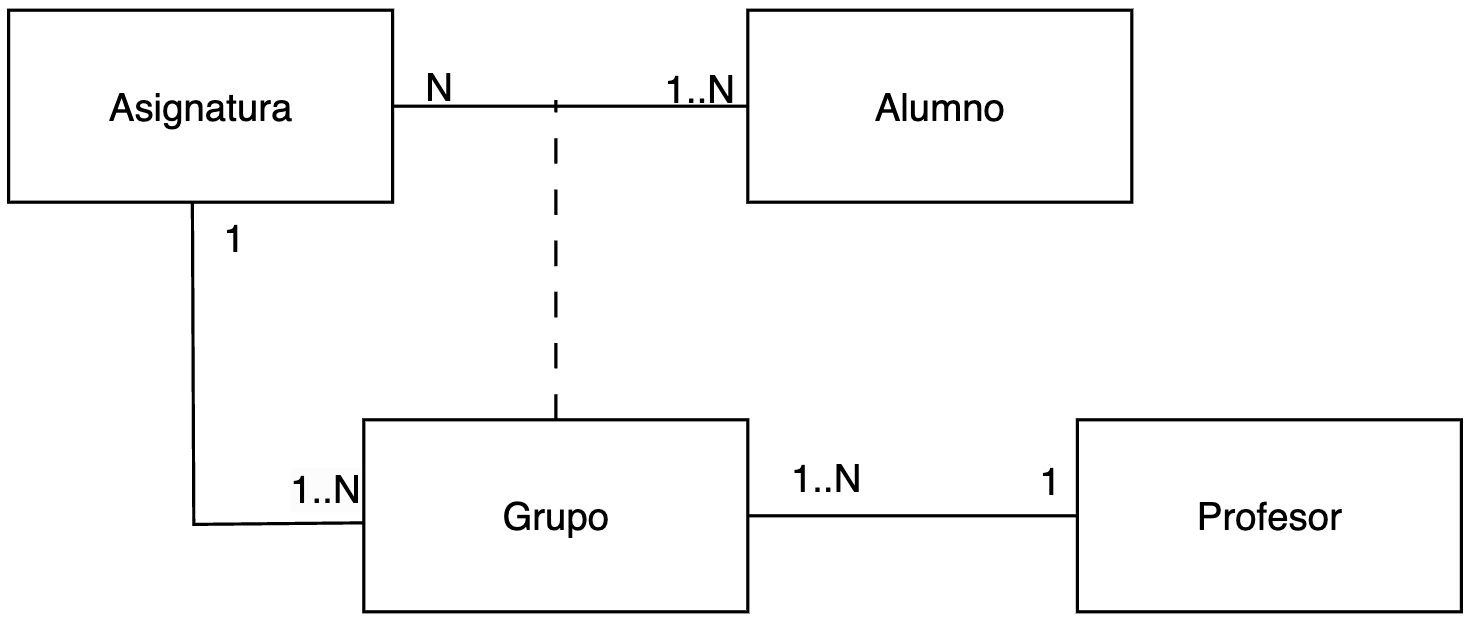
\includegraphics[width=0.8\textwidth]{assets/Junio2008_1.png.jpeg}
  \end{center}
\end{figure}
  \item Implemente las clases que aparecen, escribiendo exclusivamente los miembros imprescindibles para implementar las relaciones.
\begin{minted}[breaklines]{C++}
class Alumno; //declaración adelantada
class Grupo; //declaración adelantada
class Asignatura{
  public:
    //Relación con la clase Alumno
    typedef std::map<Alumno*,Grupo*>Alumnos;
    //Como la minima Multiplicidad es 1, lo inicializamos en el constructor
    Asignatura(Alumno& a, Grupo& g){
      setAlumno(a,g);
      setGrupo(g);
    }
    void setAlumno(Alumno& a, Grupo& g)noexcept{
      alumnos.insert(std::make_pair(&a,&g));
    }
    const Alumnos& getAlumnos()const noexcept{
      return alumnos;
    }


    //Relación con Grupo
    typedef std::set<Grupo*>Grupos;
    void setGrupo(Grupo& g)noexcept{
      grupos.insert(&g);
    }
    const Grupos& getGrupos()const noexcept{
      return grupos;
    }
  private:
    Alumnos alumnos;
    Grupos grupos;
};

class Alumno{
  public:
    //Relación con Asignatura
    typedef std::map<Asignatura*,Grupo*>Asignaturas;
    void setAsignatura(Asignatura& a, Grupo& g)noexcept{
      asignaturas.insert(std::make_pair(&a,&g));
    }
    const Asignaturas& getAsignaturas()const noexcept{
      return asignaturas;
    }
  private:
    Asignaturas asignaturas;
};

class Profesor; //declaración adelantada
class Grupo{
  public:
    //Como la multiplicidad minima es 1, lo inicializamos en el ctor
    Grupo(Asignatura& a,Profesor& p):a_(&a),p_(&p){}
    void setAsignatura(Asignatura& a)noexcept{
      a_ = &a;
    }
    void setProfesor(Profesor& p)noexcept{
      p_= &p;
    }
    const Asignatura& getAsignatura()const noexcept{return *a_;}
    const Profesor& getProfesor()const noexcept{return *p_;}
  private:
    Asignatura* a_;
    Profesor* p_;
};

class Profesor{
  public:
    //Relación con Grupo
    typedef std::set<Grupo*>Grupos;
    //Como la multiplicidad minima es 1, lo inicializamos en el ctor
    Profesor(Grupo& g){
      setGrupo(g);
    }
    void setGrupo(Grupo&g)noexcept{grupos_.insert(&g);}
    const Grupos& getGrupos()const noexcept{return grupos_;}
  private:
    Grupos grupos_;
};
  
\end{minted}
\end{enumerate}

\underbar{\textbf{\large Ejercicio 4:}} Sea \textit{Figura} una clase abstracta de la que derivan las clases \textit{Circulo}, \textit{Triangulo}, \textit{Cuadrado} y otras. Supongamos que existe una función para rotar figuras definida como sigue:
\begin{center}
  \begin{lstlisting}[frame = single]
void rotar(const Figura& fig) {
  if (typeid(fig) == typeid(Circulo)) { 
      // no hacer nada
  }
  else if (typeid(fig) == typeid(Triangulo)) {
    // rotar triangulo
  }
  else if (typeid(fig) == typeid(Cuadrado)) {
      // rotar cuadrado
  }
 // y otras
}
  \end{lstlisting}
\end{center}

\begin{enumerate}[label = \alph*)]
  \item Ponga un ejemplo de la función rotar.

\begin{minted}[breaklines]{C++}
int main(){
  //Creamos las figuras:
  Circulo circulo;
  Triangulo triangulo;
  Cuadrado cuadrado;

  //Llamamos al método rotar
  rotar(circulo);
  rotar(triangulo);
  rotar(cuadrado);

  return 0;
}
\end{minted}
  \item ¿Cree que esta es la mejor forma de implementar la rotación de figuras? Razone la respuesta. En caso negativo, describa cómo mejorarla y emplee el ejemplo anterior para mostrar la diferencia de uso.
  
  No. Si nos fijamos en el método rotar estamos comparando tipos de datos, es decir, al comparar el tipo de dato de la figura entrante con el tipo de dato triángulo, por ejemplo, vemos que ``devuelve'' (rotar triángulo), es decir, aun teniendo una clase abstracta como es Figura no estamos aplicando polimorfismo, por tanto, hemos encontrado una manera mejor y más eficiente que la comparación de tipo de datos (que es algo muy costoso).\\

  Vamos a ver como quedaría:
  \begin{minted}[breaklines]{C++}
class Figura{
  public:
    //tenemos que convertirla en interfaz
    virtual void rotar()=0;
    virtual ~Figura() = default;
};
class Circulo:public Figura{
  public:
    virtual void rotar()noexcept override{
      //no hace nada
    }
};
class Triangulo:public Figura{
  public:
    virtual void rotar()noexcept override {
      cout<<"Rotar Triangulo"<<endl;
    }
};
class Cuadrado:public Figura{
  public:
    virtual void rotar()noexcept override {
        cout<<"Rotar Cuadrado"<<endl;
      }
};

int main(){
  //Creamos las figuras
  Circulo circulo;
  Cuadrado cuadrado;
  Triangulo triangulo;
  
  circulo.rotar();
  cuadrado.rotar();
  triangulo.rotar();
}
  \end{minted}
\end{enumerate}